\documentclass{article}
\usepackage{spconf,amsmath,amssymb,graphicx,booktabs,array,microtype,dblfloatfix,float}
\graphicspath{{figures_icassp/}{figures_nested/}}
% Automatically generated from outputs/icassp_primary/summary.csv.
\newcommand{\PixelFisherRange}{0.277--0.520}
\newcommand{\CaseSpearmanRange}{0.890--0.966}
\newcommand{\NAURCRange}{0.024--0.092}
\newcommand{\RRRFiftyRange}{19.3--52.1\%}

% Automatically generated from outputs/shared_error_stress/summary.csv.
\newcommand{\StressMaeIncrease}{14.9\%}
\newcommand{\StressTargetIncrease}{28.6\%}
\newcommand{\StressSharedChange}{0.0\%}
\newcommand{\StressCommitteeMaeIncrease}{11.8\%}

\newcommand{\NestedInteractionCount}{561,492}
\newcommand{\NestedRetainedCount}{1,320}
\newcommand{\NestedBaselineNAURC}{0.077}
\newcommand{\NestedTriageNAURC}{0.052}
\newcommand{\NestedLowNAURC}{0.050}
\newcommand{\NestedBaselineRho}{0.884}
\newcommand{\NestedTriageRho}{0.911}
\newcommand{\NestedLowRho}{0.908}
\newcommand{\NestedBaselineRRR}{21.9\%}
\newcommand{\NestedTriageRRR}{21.4\%}
\newcommand{\NestedLowRRR}{21.6\%}
\newcommand{\NestedDeltaNAURC}{-0.026}
\newcommand{\NestedDeltaNAURCLo}{-0.063}
\newcommand{\NestedDeltaNAURCHi}{-0.001}
\newcommand{\NestedAttrAdv}{0.060}
\newcommand{\NestedAttrWithin}{0.126}
\newcommand{\NestedAttrTop}{27.3\%}
\newcommand{\NestedMeanNeural}{0.08}
\newcommand{\NestedLowMeanNeural}{0.04}
\newcommand{\PhysicalMatchedRecords}{1,518}

\setlength{\textfloatsep}{6pt plus 2pt minus 2pt}
\setlength{\dbltextfloatsep}{6pt plus 2pt minus 2pt}
\setlength{\floatsep}{5pt plus 2pt minus 2pt}
\setlength{\intextsep}{5pt plus 2pt minus 2pt}
\setlength{\tabcolsep}{2.7pt}
\renewcommand{\arraystretch}{0.94}
\makeatletter
\let\oldthebibliography\thebibliography
\renewcommand{\thebibliography}[1]{\oldthebibliography{#1}\setlength{\itemsep}{11.8pt plus 0.6pt minus 0.5pt}\setlength{\parsep}{0pt}\setlength{\parskip}{0pt}}
\makeatother

\title{MULTISCALE RELIABILITY RANKING OF MRI SLICE INTERPOLATION\\
VIA TARGET-TO-COMMITTEE AND PHYSICAL-PLANE DISAGREEMENT}
\name{Anonymous Authors}
\address{Anonymous submission}

\begin{document}
\ninept
\maketitle

\begin{abstract}
Cohort-average fidelity cannot identify which MRI slice interpolation should be reviewed when the missing target is unavailable. We study two ground-truth-free ranking signals from deterministic outputs: target-to-committee disagreement, which excludes the target reconstructor, and same-target consistency on physical planes generated at multiple interpolation factors. Ground truth defines only retrospective error labels. Experiments include 115 IXI, 24 fastMRI-brain, and 22 eight-fold out-of-fold NingXia T2 examinations; the latter two are evaluated at $\times2/\times4/\times6$. On nine fixed NingXia factor--target profiles, physical consistency changes mean nAURC from \NestedBaselineNAURC\ to \NestedTriageNAURC\ and Spearman correlation from \NestedBaselineRho\ to \NestedTriageRho; the profile-aligned paired nAURC difference is \NestedDeltaNAURC\ [\NestedDeltaNAURCLo, \NestedDeltaNAURCHi]. Conversely, nested target/scale-specific selection over \NestedInteractionCount\ registered score--committee interactions does not outperform the frozen baseline, and calibrated target attribution remains weak. Shared errors cancel from cross-model disagreement. These scores rank selective review; neither is a calibrated probability or clinical guarantee.
\end{abstract}

\begin{keywords}
MRI interpolation, reliability ranking, selective review, model disagreement, multiscale consistency
\end{keywords}

\section{Introduction}
Through-plane interpolation densifies sparse MRI stacks for visualization, registration, and volumetric processing. Modern methods model inter-slice context or adapt restoration transformers \cite{song2024i3net,liang2021swinir,chen2022hat}, yet are usually compared by cohort-average PSNR, SSIM, or MAE. Such summaries cannot identify an unreliable examination after the missing target slice becomes unobservable.

Model-internal uncertainty uses stochastic inference, repeated training, heteroscedastic objectives, test-time augmentation (TTA), or learned error prediction \cite{gal2016dropout,lakshminarayanan2017deepensembles,kendall2017uncertainties,wang2018tta,edupuganti2021uqmri,hu2021predict,zhang2024trainingfree}; no-reference MRI quality assessment instead targets perceptual quality or acquisition artifacts \cite{stepien2022nriqa}. Our operational setting assumes only deterministic interpolator outputs and asks whether they rank examinations for selective review \cite{elyaniv2010selective,geifman2019selectivenet,ding2020aurc}. Heterogeneous outputs provide cross-model evidence, while reconstructions of the same source stack at known factors provide a second signal when their generated planes coincide physically.

We contribute: (1) a target-excluded reliability-ranking protocol augmented by physical-plane cross-scale consistency; (2) a leakage-controlled evaluation with common-support fidelity, \NestedInteractionCount\ registered score--committee interactions, eight-fold nested selection, calibrated target attribution, and profile-aligned bootstrap; and (3) empirical boundaries showing that fixed disagreement transfers better than high-flexibility adaptive selection, while shared errors remain invisible. We claim error association and review ranking, not posterior uncertainty, diagnostic correctness, or clinical safety.

\section{Method}
\subsection{Target-to-committee disagreement}
Let $x$ be observed sparse-slice context, $y$ the unobserved dense target, and $\hat y_m=f_m(x)$ the output of target interpolator $m$. For available identities $\mathcal B$, define $\mathcal C_m=\{b\in\mathcal B:b\neq m\}$. All outputs must share case identity, source-intensity representation, affine, orientation, voxel grid, and generated-slice convention. At generated voxel $i$, the frozen map is
\begin{equation}
 U_m(i)=\mathop{\mathrm{median}}_{b\in\mathcal C_m}|\hat y_m(i)-\hat y_b(i)|.
 \label{eq:target}
\end{equation}
This is median target-to-member disagreement, not statistical median absolute deviation or posterior variance. Let $\mathcal G_r$ be slices generated at factor $r$. The deployment mask and examination score are
\begin{align}
 M_m(i)&=\mathbf1[|\hat y_m(i)|>0.01\max_{j\in\mathcal G_r}|\hat y_m(j)|],\nonumber\\
 s_m&=\frac{\sum_{i\in\mathcal G_r}M_m(i)U_m(i)}{\sum_{i\in\mathcal G_r}M_m(i)}. \label{eq:case}
\end{align}
Ground truth is inaccessible to Eqs.~\eqref{eq:target}--\eqref{eq:case}. Bank-union and observed-input masks, upper-tail pooling, gradient/Laplacian domains, relative differences, member weighting, trimming, and subset committees are registered alternatives.

\begin{figure}[!t]
 \centering
 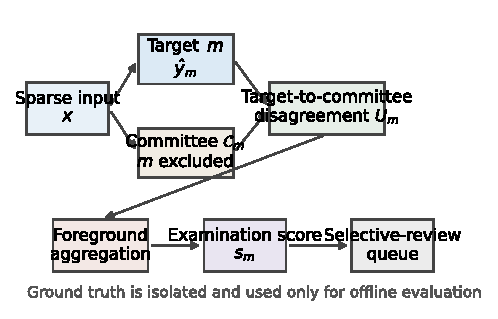
\includegraphics[width=0.98\columnwidth]{figure_framework_outlined.pdf}
 \caption{Ground-truth-free scoring and offline evaluation. The named target is excluded from its committee; missing targets are revealed only to the evaluator.}
 \label{fig:framework}
\end{figure}

\subsection{Physical cross-scale consistency}
Array depth alone does not determine whether factors can be compared. For NIfTI affine $A$, slice $z$ has world-plane origin $p(z)=A_{1:3,4}+A_{1:3,3}z$. For factors $r\neq r'$, we retain only planes generated in both reconstructions whose origins agree within $10^{-3}$ mm; no resampling is introduced. The same-target physical signal is
\begin{equation}
 C_m(p)=\mathop{\mathrm{median}}_{r\neq r'}|\hat y_m^{(r)}(p)-\hat y_m^{(r')}(p)|,
 \label{eq:physical}
\end{equation}
aggregated over a union foreground. We evaluate Eq.~\eqref{eq:physical} alone and the pre-defined rank hybrid $h_m=\tfrac12\operatorname{rank}(s_m)+\tfrac12\operatorname{rank}(C_m)$. Physical consistency requires reconstructions at multiple known factors, so it is most natural for cached retrospective audits; it is not a cheaper substitute for a single online reconstruction.

\subsection{Failure boundary and selective review}
Write $\hat y_b=y+c+\epsilon_b$, where $c$ is shared error and $\epsilon_b$ member-specific. Then $\hat y_m-\hat y_b=\epsilon_m-\epsilon_b$: disagreement responds to model-specific separation but exactly cancels any identical perturbation applied to all outputs. Consensus therefore cannot certify correctness.

For offline error $E_j$, examinations are retained by increasing score. At coverage $q$, $R(q)$ is retained mean MAE and $\mathrm{RRR}(q)=[R_{\rm random}-R(q)]/R_{\rm random}$. We report Spearman $\rho$ and $\mathrm{nAURC}=(\mathrm{AURC}-\mathrm{AURC}_{\rm oracle})/(\mathrm{AURC}_{\rm random}-\mathrm{AURC}_{\rm oracle})$, where zero is oracle and one expected random review. Coverage always means retained fraction.

\section{Experiments}
\subsection{Data, models, and governance}
The factor-four study uses IXI (115 examinations) \cite{ixi}, fastMRI-brain (24) \cite{zbontar2018fastmri}, and an internal NingXia T2 cohort (22) pooled from eight out-of-fold prediction folds. fastMRI-brain and NingXia also use the same identities at $\times2$ and $\times6$. Eleven neural reconstructors are audited: I$^3$Net, HAT, SwinIR, SAINT, SMamba-UNet, Pix2PixGAN, ResUNet, ResSRDiff, ArSSR, CycleINR, and ACVTT; linear and cubic interpolation are analytical references \cite{keys1981cubic,thevenaz2000interpolation}. All listed outputs pass case, shape, affine, finite-value, and generated-index checks.

Cross-model fidelity is recomputed on one offline ground-truth 1\% foreground and generated slices, rather than each model's own mask. Development-only composite ranks over MAE, MSE, PSNR, global SSIM, and NCC define six main targets and an architecture-constrained common bank of six neural plus two analytical members. No NingXia outer result changes these identities.

Broad screening uses IXI $\times4$ and fastMRI-brain $\times2/\times4/\times6$. We enumerate \NestedInteractionCount\ interactions over 18 intensity, structural, and pooling features, committee sizes 2--5/full, and six uniform, fidelity, diversity, combined, or trimmed weighting rules; stratified pruning retains \NestedRetainedCount. For each NingXia outer fold, the other seven folds select a target- and factor-conditioned candidate; the outer score is calibrated by its inner empirical CDF. A declared cost rank and one-standard-error simplicity rule are implemented. The first unconstrained pass and a prospectively recorded neural-peer amendment are both retained after neither transfers. Attribution calibration and relative centering are selected by matched advantage, within-case model ranking, and top-1 identification, not triage nAURC.

Every final profile contains all 22 outer predictions. We use 2,000 paired case-bootstrap replicates with fixed indices. Aggregate differences are computed within each replicate for every fixed factor--target profile and only then averaged across profiles. Thus profile bootstrap samples are never flattened. Failure-decile AUROC/AUPRC remain secondary.

\section{Results}
\begin{table}[!t]
 \centering
 \caption{NingXia outer-fold ranking, averaged over I$^3$Net, HAT, and SwinIR. Coverage is retained fraction; lower nAURC is better.}
 \resizebox{\columnwidth}{!}{\begin{tabular}{llccc}
\toprule
Factor & Method & $\rho$ [95\% CI] & nAURC [95\% CI] & RRR50 \\
\midrule
$\times$2 & Frozen baseline & 0.879 [0.749, 0.941] & 0.070 [0.033, 0.139] & 22.3\% \\
$\times$2 & Physical consistency & 0.878 [0.744, 0.946] & 0.075 [0.035, 0.150] & 20.6\% \\
$\times$2 & Fixed rank hybrid & 0.886 [0.757, 0.949] & 0.066 [0.030, 0.133] & 20.6\% \\
$\times$2 & Mean disagreement & 0.893 [0.770, 0.953] & 0.064 [0.028, 0.130] & 22.0\% \\
$\times$4 & Frozen baseline & 0.912 [0.820, 0.945] & 0.063 [0.031, 0.142] & 22.2\% \\
$\times$4 & Physical consistency & 0.934 [0.852, 0.964] & 0.053 [0.026, 0.096] & 21.6\% \\
$\times$4 & Fixed rank hybrid & 0.934 [0.855, 0.965] & 0.034 [0.019, 0.093] & 22.2\% \\
$\times$4 & Mean disagreement & 0.915 [0.819, 0.949] & 0.057 [0.028, 0.129] & 22.2\% \\
$\times$6 & Frozen baseline & 0.862 [0.730, 0.920] & 0.098 [0.049, 0.184] & 21.2\% \\
$\times$6 & Physical consistency & 0.922 [0.814, 0.972] & 0.026 [0.010, 0.058] & 22.0\% \\
$\times$6 & Fixed rank hybrid & 0.906 [0.792, 0.950] & 0.051 [0.024, 0.097] & 22.1\% \\
$\times$6 & Mean disagreement & 0.843 [0.704, 0.903] & 0.122 [0.062, 0.219] & 20.2\% \\
\bottomrule
\end{tabular}
}
 \label{tab:nested}
\end{table}

\begin{figure*}[!t]
 \centering
 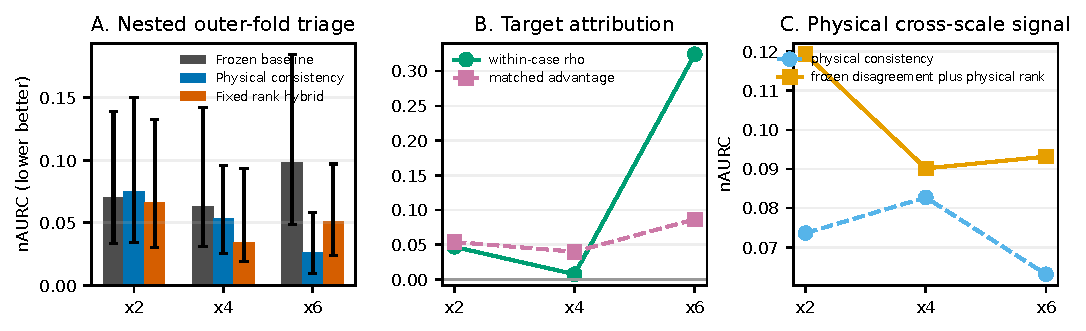
\includegraphics[width=0.98\textwidth]{nested_multiscale_results.pdf}
 \caption{Outer-fold evidence. (A) Fixed cross-model baseline, physical consistency, and their rank hybrid. (B) Attribution after inner-fold target calibration. (C) Physical consistency and hybrid across all audited targets. Error bars in (A) are profile-aligned 95\% bootstrap intervals.}
 \label{fig:nested}
\end{figure*}

\subsection{Physical consistency improves examination ranking}
All \PhysicalMatchedRecords\ audited case--target--scale-pair records contain at least one common generated physical plane. On the nine primary NingXia profiles, Eq.~\eqref{eq:physical} improves mean nAURC from \NestedBaselineNAURC\ to \NestedTriageNAURC\ and $\rho$ from \NestedBaselineRho\ to \NestedTriageRho\ (Table~\ref{tab:nested}, Fig.~\ref{fig:nested}). The profile-aligned paired nAURC change is \NestedDeltaNAURC\ [\NestedDeltaNAURCLo, \NestedDeltaNAURCHi]. The fixed hybrid has nAURC \NestedLowNAURC\ and RRR50 \NestedLowRRR; its difference from consistency alone is inconclusive. This supports complementary physical evidence, not probability calibration.

\subsection{Adaptive selection and attribution do not transfer}
The frozen baseline obtains nAURC \NestedBaselineNAURC, $\rho=\NestedBaselineRho$, and RRR50 \NestedBaselineRRR. Mean disagreement is nearly identical, so the median aggregator is not claimed as a unique algorithmic advance. In contrast, the unconstrained nested selector collapses mostly to Linear+Cubic under one-SE and obtains nAURC 0.270; requiring neural peers and adding public-development stability yields 0.299. Both failures remain registered. The result argues for a simple frozen default when labeled inner folds are tiny, rather than dataset-specific committee claims.

Target-calibrated attribution has mean matched advantage \NestedAttrAdv, within-case $\rho=\NestedAttrWithin$, and top-1 accuracy \NestedAttrTop. It is stronger at $\times6$ but weak overall; examination difficulty, rather than target identity, explains most score variation. We therefore present target attribution as a boundary, not a validated deployment claim.

\subsection{Common-support selection diagnostics}
Correcting the development support materially changes model order (Table~\ref{tab:fidelity}). HAT moves from rank 6 to 3, while SMamba-UNet, Pix2PixGAN, and SwinIR each move down one place. This demonstrates why reconstruction fidelity cannot be compared on model-specific masks. The target set is frozen from the corrected ranking, not from reliability performance.

\begin{table}[H]
 \centering
 \caption{Top-half neural targets by corrected fastMRI-brain development fidelity averaged over three factors. Old rank used model-specific masks.}
 \resizebox{0.84\columnwidth}{!}{\begin{tabular}{r l r r r}
\toprule
Rank & Model & MAE & SSIM & Old \\
\midrule
1 & i3net & 66.0 & 0.881 & 1 \\
2 & saint & 81.0 & 0.847 & 2 \\
3 & hat & 83.6 & 0.830 & 6 \\
4 & smamba\_unet & 83.9 & 0.827 & 3 \\
5 & pix2pixgan & 81.6 & 0.840 & 4 \\
6 & swinir & 84.6 & 0.823 & 5 \\
\bottomrule
\end{tabular}
}
 \label{tab:fidelity}
\end{table}

Table~\ref{tab:adaptive} separates the fixed physical result from adaptive failures. The unconstrained selector chooses almost no neural peers; the amended constraint restores learned diversity but does not restore ranking. The negative result is therefore not explained solely by cheap analytical members.

\begin{table}[H]
 \centering
 \caption{Primary-target aggregate and mean selected neural peers. Adaptive rows are nested outer-fold results.}
 \resizebox{0.96\columnwidth}{!}{\begin{tabular}{lrrrr}
\toprule
Method & $\rho$ & nAURC & RRR50 & Neural peers \\
\midrule
Frozen baseline & 0.884 & 0.077 & 21.9\% & -- \\
Physical consistency & 0.911 & 0.052 & 21.4\% & -- \\
Unconstrained nested & 0.705 & 0.270 & 19.9\% & 0.08 \\
Amended nested & 0.670 & 0.299 & 19.4\% & 2.14 \\
\bottomrule
\end{tabular}
}
 \label{tab:adaptive}
\end{table}

\subsection{Shared errors, cost, and scope}
In the controlled IXI stress test, maximum-strength target-only corruption raises disagreement by \StressTargetIncrease, whereas applying the identical corruption to all outputs changes disagreement by only \StressSharedChange\ despite increasing reconstruction error (Fig.~\ref{fig:stress}). This verifies common-mode invariance, not clinical realism.

\begin{figure}[H]
 \centering
 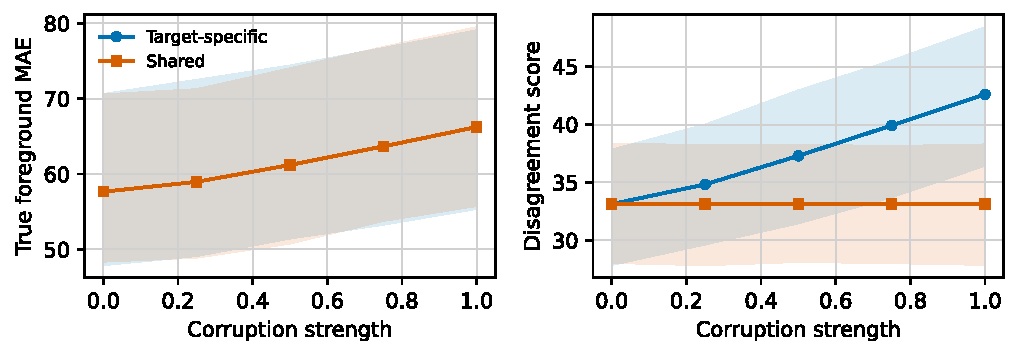
\includegraphics[width=0.96\columnwidth]{shared_error_stress_outlined.pdf}
 \caption{Target-specific corruption raises error and disagreement; identical shared corruption raises error while cancelling from cross-model differences. Bands are 95\% bootstrap intervals.}
 \label{fig:stress}
\end{figure}

Stored-output cross-model scoring takes 1.18 s mean per examination on CPU with 0.89 GiB peak RSS. Physical consistency adds comparisons but, online, requires two additional factor-specific executions of the target model; the hybrid also requires committee outputs. Thus cross-model scoring suits cached audits, while physical consistency trades more reconstruction cost for improved multiscale ranking.

\section{Discussion and Conclusion}
Case ranking is stronger than voxel localization because foreground aggregation suppresses local noise while preserving between-examination severity. Physical consistency adds a distinct signal: it observes whether one reconstructor changes on the same world plane as sampling context changes. Its success does not rescue target attribution, and a high score may still flag correct but unusual detail.

The evidence has three levels. The original median disagreement, mask, and review metric were frozen before multiscale analysis. Physical matching and the 50/50 rank hybrid were specified before world-coordinate results were computed, so their nine-profile comparison is an evaluation of fixed formulas rather than per-profile selection. By contrast, the amended adaptive selector was introduced after diagnosing the analytical-only collapse; its complete outer results are retained but interpreted only as an exploratory sensitivity. This distinction prevents a negative first finalist from being silently replaced.

The physical score is attractive when a benchmark, model-comparison service, or retrospective audit already stores multiple factors. In a single-factor online system it requires two extra executions of the target reconstructor. Cross-model disagreement instead requires peer models, but analytical members are inexpensive and cached neural predictions amortize reconstruction cost. The hybrid has the highest online burden and should be used only when the observed ranking gain justifies this cost. None of the scores changes the reconstructed volume or autonomously rejects an examination; it only orders a review queue whose operating coverage is set by available human capacity.

\begin{table}[H]
 \centering
 \caption{Operational interpretation. All signals are ground-truth-free at scoring time.}
 \resizebox{\columnwidth}{!}{\begin{tabular}{llll}
 \toprule
 Signal & Required outputs & Main evidence & Structural blind spot \\
 \midrule
 Cross-model & target + peers & target separation & shared model error \\
 Cross-scale & target at factors & context sensitivity & scale-stable error \\
 Rank hybrid & both sets & complementary order & both common modes \\
 \bottomrule
 \end{tabular}}
 \label{tab:operations}
\end{table}

The factor dependence is informative rather than a reason to choose a different rule after testing. At $\times2$, many generated planes lie close to observed anchors, and cross-model mean disagreement is already competitive. At $\times6$, context is sparser and the frozen cross-model baseline degrades, while the same-target physical score remains strongly associated with examination error. We interpret this as evidence that sensitivity to sampling context becomes useful as the interpolation gap grows. It does not imply that one factor's reconstruction is a reference for another: both can be wrong, and only pairwise inconsistency is observed.

The three evaluation tasks must remain separate. Examination triage pools evidence over one target's volume and is the only task strongly supported across all factors. Target attribution compares calibrated scores across reconstructors within one examination; its modest top-1 accuracy is not sufficient to identify a failed model automatically. Shared difficulty summarizes whether many reconstructors struggle on the same case, but by construction cannot assign responsibility. A deployed interface should therefore expose the target identity and score provenance, not collapse these outputs into an unlabeled ``uncertainty'' value.

The nested failures also change how committee refinement should be interpreted. A member can improve reconstruction fidelity, add architectural diversity, or reduce deployment cost without improving risk ordering. With only 18--20 inner examinations in each outer run, hundreds of close candidates are weakly identified even after family-wise pruning. The one-standard-error rule controls formula complexity but cannot create information absent from the labels. Larger development cohorts or fewer pre-declared alternatives are needed before target-conditioned committees can replace a frozen default.

For practical monitoring, member identities, factor, affine hash, normalization version, mask type, and raw score should be logged with every queue entry. Software upgrades or acquisition changes can then be detected as score-distribution drift before changing a referral threshold. Thresholds should be set from review capacity on development data and frozen prospectively; our retrospective curves compare rankings rather than recommending a universal operating point. When only one model and one factor can be run, TTA or a validated model-internal predictor may be more appropriate than either signal in Table~\ref{tab:operations}.

Limitations are substantive. Shared blur, deletion, bias, or preprocessing failure can fool all members; correlated training data reduce committee diversity; masks can omit suppressed tissue; fastMRI-brain and NingXia are small; evidence is T2 brain MRI; and cross-scale scoring requires multiple reconstructions. MAE is not diagnostic harm, no reader or downstream study is available, and neither score is calibrated. We conclude that target-to-committee disagreement is a reproducible frozen review baseline and physical-plane consistency can strengthen multiscale examination ranking. Adaptive committee selection needs larger development cohorts; neither consensus nor consistency guarantees clinical correctness.

\clearpage
\bibliographystyle{IEEEbib}
\bibliography{references}
\end{document}
